% \begin{frame}{A Theory of Onset Temperature in 2D: The Role of Entropy}

% \begin{figure}
%     \centering
%     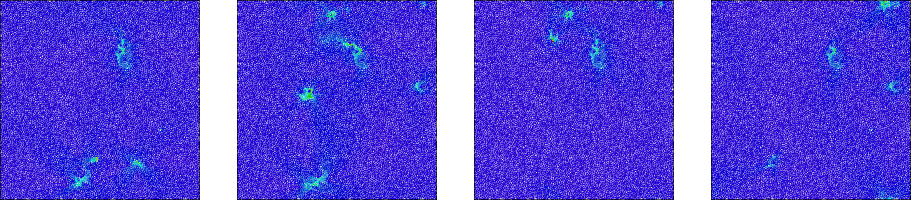
\includegraphics[height=0.375\textheight]{3.d-kt_geomcharges/excs.png}
%     \caption{Mobile regions at $T \approx 0.53 T_\mathrm{o}$ and $t \ll \tau_\mathrm{eq}$, sampled from trajectories starting from the same initial configuration $\{\* R_0^\alpha\}$ $\to$ \textbf{isoconfigurational ensemble} (Widmer-Cooper, Harrowell, Fynewever, \textit{PRL}, 2004).} %
% \end{figure}
% % \begin{columns}
% % \begin{column}{0.5\linewidth}
% % \begin{itemize}
% %     \item T
% % \end{itemize}
% % \end{column}

% % \begin{column}{0.5\linewidth}
% %hint for onset temperature $T_\mathrm{o}$ lies in the mathematical model for the localized pure-shear excitation
% \vspace{-14pt}
% \begin{itemize}
% \item<2-> The free-energy of formation for a localized pure-shear excitation
% \begin{equation*}
% \onslide<3->{\Delta F_\mathrm{f} = \underbrace{E_\mathrm{c}}_{\substack{\text{Strain elastic} \\ \text{energetic cost}}}} \onslide<4->{-\underbrace{2 k_\mathrm{B} T \ln \left(\sqrt{2 \pi} \frac{R}{R_\mathrm{exc}} \right)}_{\substack{\text{Entropy gain} \\ \text{(translation + orientation)}}}} \onslide<5->{< 0} 
% \end{equation*}
% \onslide<5->{In the thermodynamic limit ($R \to \infty$), excitations are always favored (\textit{no transition})!} 
% %\item<7-> \textbf{Analogy to electrostatics: geometric dipole} with dipole-moment vector $\mathbf{d}$, where {\large $|\* d| \sim \epsilon_\mathrm{c}$} 
% \end{itemize}
% % \end{column}
% % \end{columns}

% % \begin{figure}
% % \vspace{-9pt}
% % \begin{overprint}

% % \onslide<2-7>\centering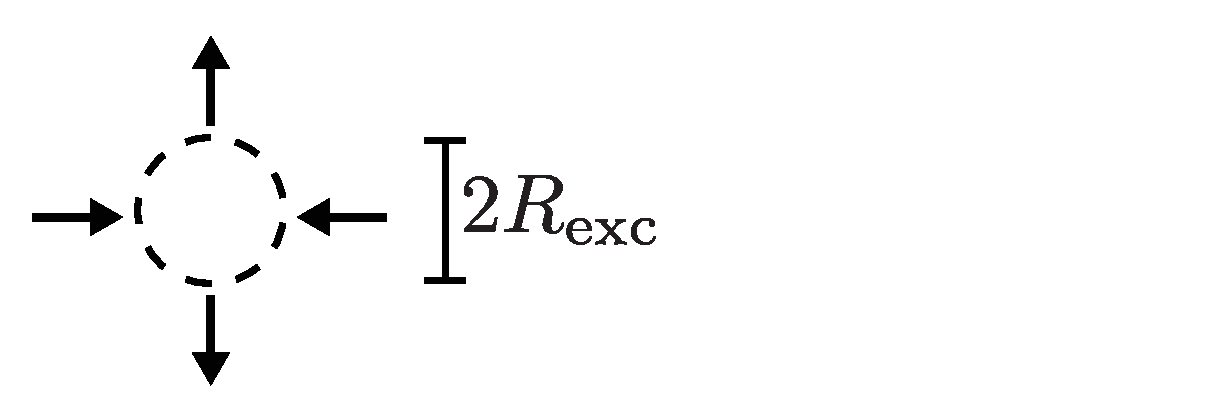
\includegraphics[width=0.75\linewidth]{3.d-kt_geomcharges/chargesequiv-0.pdf}%\caption{Testing}

% % \onslide<8>\centering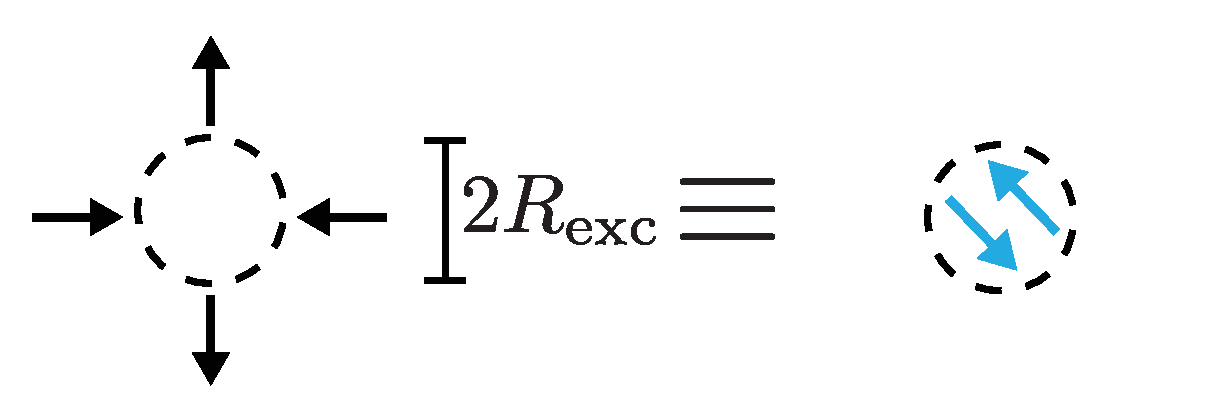
\includegraphics[width=0.75\linewidth]{3.d-kt_geomcharges/chargesequiv-1.pdf}%\caption{Testing}

% % %\onslide<8->\centering\includegraphics[width=0.75\linewidth]{3.d-kt_geomcharges/chargesequiv-2.pdf}


% % \end{overprint}
    
% % \end{figure}
    
% \end{frame}


\begin{frame}{A Theory of Onset Temperature in 2D: Geometric Charges \& Energy-Entropy Framework}

\begin{columns}[T]
\begin{column}[T]{0.5\textwidth}

\begin{block}{\centering \large Geometric Charges}
Mathematical analogy (unique to 2D) between elastic excitations and electrostatic multipoles
\end{block}

\begin{figure}
\centering\includegraphics[width=0.9\linewidth]{c.2-kt_geomcharges_1/chargesequiv-2.pdf}
\vspace{-5pt}
\includegraphics[width=0.6\linewidth]{c.2-kt_geomcharges_1/dipolemag.pdf}
\caption{Pure-shear excitation as bound state of \textbf{geometric dipoles}}
\end{figure}

\end{column}

\begin{column}[T]{0.5\textwidth}

\begin{block}{\centering \large Energy-Entropy Framework}
Free energy of formation for localized excitations
\end{block}

\vspace{0.3em}

\begin{equation*}
\underbrace{\Delta F_\mathrm{f}}_{\substack{\text{Free energy of} \\ \text{formation}}} = \underbrace{ \frac{d_{\mathrm{c}}^{2} Y^{\mathrm{IS}}}{8 \pi} \ln \left(\frac{R}{R_{\mathrm{exc}}}\right) }_{\substack{\text{Elastic energy cost}}} - \underbrace{2 k_\mathrm{B} T \ln \left(\sqrt{2 \pi} \frac{R}{R_\mathrm{exc}} \right)}_{\substack{\text{Entropy gain}}}
\end{equation*}

\vspace{0.5em}

\begin{itemize}
\item \textbf{Low-$T$:} Bound geometric dipoles (solid behavior)
\item \textbf{High-$T$:} Free dipoles (fluid behavior)  
\item \textbf{Critical condition:} Balance of energy vs entropy
\end{itemize}

\end{column}
\end{columns}

\vspace{0.5em}

\begin{block}{\centering Key Insight}
Localized excitations are \textbf{bound states of geometric dipoles} that undergo a binding-unbinding transition at $T_\mathrm{o}$
\end{block}

\end{frame}

% \begin{frame}{A Theory of Onset Temperature in 2D: Energy-Entropy Arguments}
% % \begin{columns}
% % \begin{column}{0.5\linewidth}
% % \begin{itemize}
% %     \item T
% % \end{itemize}
% % \end{column}

% % \begin{column}{0.5\linewidth}
% %hint for onset temperature $T_\mathrm{o}$ lies in the mathematical model for the localized pure-shear excitation
% \begin{itemize}
% \item<2-> The free-energy of formation for a localized pure-shear excitation
% \begin{equation*}
% \onslide<3->{\Delta F_\mathrm{f} = \underbrace{E_\mathrm{c}}_{\substack{\text{Strain elastic} \\ \text{energetic cost}}}} \onslide<4->{-\underbrace{2 k_\mathrm{B} T \ln \left(\sqrt{2 \pi} \frac{R}{R_\mathrm{exc}} \right)}_{\substack{\text{Entropy gain} \\ \text{(translation + orientation)}}}} \onslide<5->{< 0} 
% \end{equation*}
% \onslide<5->{In the thermodynamic limit ($R \to \infty$), excitations are always favored (\textit{no transition})!} 

% \onslide<6->{
% \begin{block}{\centering The Nature of Excitations at Finite-$T$}
% \onslide<7->{ Localized pure-shear excitations are emergent objects at low-$T$} \onslide<8->{ $\to$ a bound state of two excitations (Moshe, et al., \textit{Proc. Natl. Acad. Sci. U.S.A.} 2015) }
% \end{block}
% }
% %\item<7-> \textbf{Analogy to electrostatics: geometric dipole} with dipole-moment vector $\mathbf{d}$, where {\large $|\* d| \sim \epsilon_\mathrm{c}$} 
% \end{itemize}
% % \end{column}
% % \end{columns}

% \begin{figure}
% \vspace{-9pt}
% \begin{overprint}

% \onslide<2-7>\centering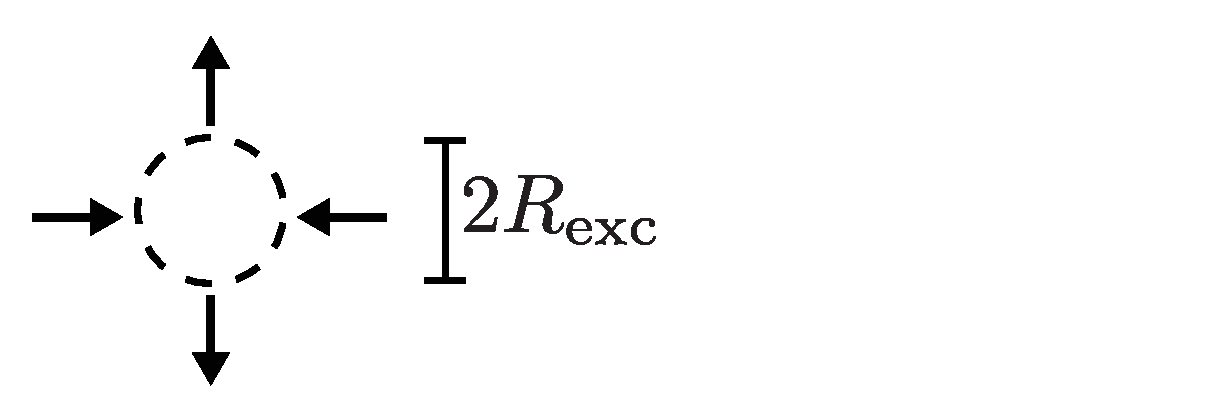
\includegraphics[width=0.75\linewidth]{3.d-kt_geomcharges/chargesequiv-0.pdf}%\caption{Testing}

% \onslide<8>\centering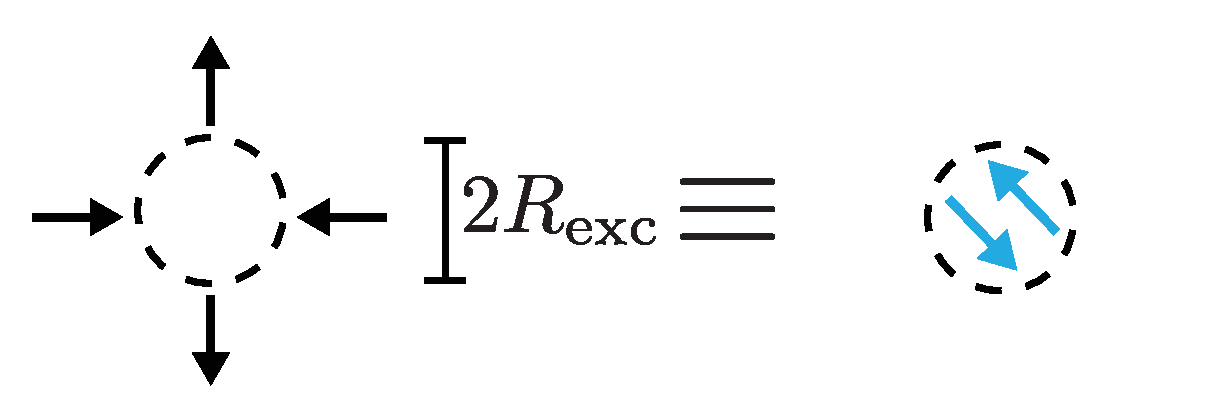
\includegraphics[width=0.75\linewidth]{3.d-kt_geomcharges/chargesequiv-1.pdf}%\caption{Testing}

% %\onslide<8->\centering\includegraphics[width=0.75\linewidth]{3.d-kt_geomcharges/chargesequiv-2.pdf}


% \end{overprint}
    
% \end{figure}
    
% \end{frame}


% \begin{frame}{A Theory of Onset Temperature in 2D: Excitations as a Bound State}
% % \begin{columns}
% % \begin{column}{0.5\linewidth}
% % \begin{itemize}
% %     \item T
% % \end{itemize}
% % \end{column}

% \begin{figure}
% \vspace{-9pt}
% \begin{overprint}
% \onslide<1-10>\centering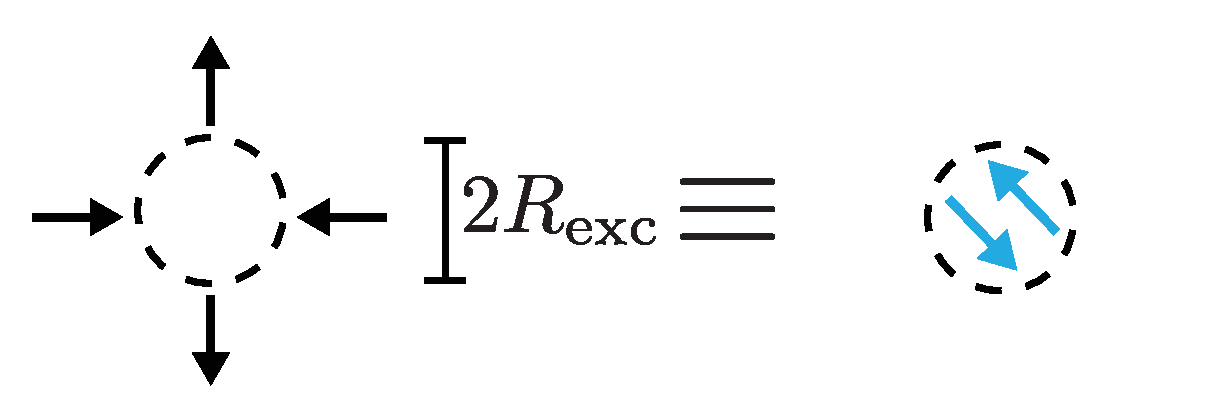
\includegraphics[width=0.5\linewidth]{3.d-kt_geomcharges/chargesequiv-1.pdf}
% \onslide<11->\centering\includegraphics[width=0.5\linewidth]{3.d-kt_geomcharges/chargesequiv-2.pdf}\hspace{3pt}\raisebox{12pt}{\includegraphics[width=0.35\linewidth]{3.d-kt_geomcharges/dipolemag.pdf}}
% \end{overprint}
% %\begin{equation*}

% %\end{equation*}
% \end{figure}
% \vspace{-7pt}
% % \begin{column}{0.5\linewidth}
% %hint for onset temperature $T_\mathrm{o}$ lies in the mathematical model for the localized pure-shear excitation
% \begin{itemize}
% \item Mathematical analogy (unique to 2D) between elastic defects, i.e., sources of singularities in stress/strain, with multipoles in electrostatics %The free-energy of formation for a localized pure-shear excitation:
% \vspace{8pt}
% \begin{table}[h]
% \begin{tabular}{cc}
% \hline\hline
% Electrostatics  & 2D Elasticity  \\ \hline
% \onslide<2->{Electric field $E_i=-\phi_{,i}$} & \onslide<6->{Stress field $T_{ij} = \chi_{,kk} \delta_{ij}-\chi_{,ij}$}  \\
% \onslide<2->{Potential function $\phi$} & \onslide<7->{Airy stress function $\chi$} \\
% \onslide<3->{Charge distribution $\rho$} & \onslide<8->{Incompatibility source $\eta$}  \\
% \onslide<4->{Dielectric constant $\varepsilon$}    & \onslide<9->{Young's modulus $Y$}   \\
% \onslide<5->{Poisson's equation $-\varepsilon \nabla^2 \phi = \rho$} & \onslide<10->{$\frac{1}{Y} \nabla^4 \chi = \eta$ } \\
% \hline\hline
% \end{tabular}
% %\end{ruledtabular}
% \end{table}
% \vspace{8pt}
% \item<12-> A pure-shear excitation is a bound state of \textbf{geometric dipoles} \pause $ \to$ 2D elastic defects as geometric charges (Moshe, et al. \textit{Proc. Natl. Acad. Sci. U.S.A.} 2015).
% \end{itemize}
% % \end{column}
% % \end{columns}

% \end{frame}